\section{Classification}
\label{sec:exp-clf}
    \subsection{Overview}
    \label{subsec:exp-clf-overview}
        In this section, parameters that alter the training set of data and those which affect the training process itself will be experimentally optimised to produce near-optimum performance. An exhaustive grid search, without consideration of post-processing, would require training and testing of each classifier hundreds of thousands of times, taking tens of thousands of days of computing time. Instead, an iterative approach will be taken, depicted in figure \ref{fig:exp-clf-overview-opt}. 
        \newcommand{\optnode}[5]{
    % supernode id, find content, assume content, found content, position 
    \node (#1-find) [smallamber,minimum height=0.1cm ,text width=1.6cm,minimum width = 2cm #5] {\specialcell{#2}};
    \node (#1-assume) [smalldarkbyzantium,minimum height=0.1cm, text width=1.6cm, minimum width = 2cm, below=0.15cm of #1-find] {\specialcell{#3}};
    \node (#1-found) [smallazure,minimum height=0.1cm, text width=1.6cm, minimum width = 2cm, below=0.15cm of #1-assume] {\specialcell{#4}};
    \begin{pgfonlayer}{background}
        \node(#1)[bigblush] [fit = (#1-find) (#1-found)] {};
    \end{pgfonlayer}
}
\def\dist{0.3cm}
\begin{tikzfig}{fig:exp-clf-overview-opt}{Optimisation and iteration of pre-classification pipeline.}{\tiny}
    
    \optnode{feats}{choose features}{balance classes\\normalise audio\\training labels\\classifier params}{normalise features\\testing label}{}
    \optnode{balance}{balance classes}{normalise audio\\training labels\\classifier params}{normalise features\\testing label\\chosen features}{, right=\dist of feats-find}
    \optnode{normaud}{normalise audio}{training labels\\classifier params}{normalise features\\testing label\\chosen features\\balance classes}{, right=\dist of balance-find}
    \optnode{labels}{choose train labels}{classifier params}{normalise features\\testing label\\chosen features\\balance classes\\normalise audio}{, right=\dist of normaud-find}
    \optnode{clf}{classifier params}{none}{normalise features\\testing label\\chosen features\\balance classes\\normalise audio\\chosen train labels}{, right=\dist of labels-find}
    \optnode{done}{none}{none}{normalise features\\testing label\\chosen features\\balance classes\\normalise audio\\chosen train labels\\classifier params}{, right=\dist of clf-find}
    
    \optnode{key}{optimising}{assumed}{chosen/estimated}{, left=3cm of balance-find}

    \draw[arrow](feats)--(balance);
    \draw[arrow](balance)--(normaud);
    \draw[arrow](normaud)--(labels);
    \draw[arrow](labels)--(clf);
    \draw[arrow](clf)--(done);
    \draw [arrow] (done-found.east) -| (12.85,-3.37) |- (-1.4,-3.37)  node[near end,above]{iterate}-| (-1.4,-2) |- (feats-assume.west);

    
\end{tikzfig}
        \twN{change order so classifier params after feature slection}
        For each stage, one parameter/set of parameters is locally optimised whilst making initial assumptions about the others. These first-iteration optimised parameters are fed back to the start of the pipeline, replacing the initial assumptions and running the procedure until convergence is achieved. This approach means that for each iteration, each classifier will only have to be trained/tested $\sim250$ times. Optimisation for every stage in the pipeline is done by methods of cross-validation; the model with the highest performing hyperparameter combination is chosen and then tested on the 'unseen', results of which are presented in tables throughout this section. Model selection decisions will \textit{not} be influenced by test results on unseen data for reasons discussed in section \ref{subsec:exp-clf-xval}. This section is strongly linked with sections \ref{sec:pl-data} to \ref{sec:pl-clf}, which detail the mathematics and implementation specifics of the procedures highlighted here.
        
        Performance will be evaluated over each of the chosen classifiers using the metrics F1 score, area under the receiver-operator curve (AUC-ROC), area under the precision-recall curve (AUC-PR), true positive rate (TPR), and the true negative (TNR) rate. These metrics have been chosen as they represent important classifier characteristics in a compact form, convenient for comparing many results. More details regarding metrics can be found in section \ref{sec:pl-test}. 

        \twN{maybe remove iteration and mention in ideal situation would do this, still produces pretty optimised pipeline}
        % limitations of this approach, initial parameter selection will 'steer' it down a specific route which iteration wont solve but only possible approach, could be overcome by randomly seeding initial assumptions then iterating through those pipelines but still too much computation required
      
     
    \subsection{Classifier Selection}
    \label{subsec:exp-clf-select}
        Of the implemented classifiers [naive bayes, gaussian mixture model, knn, gaussian processes, svm, random forest, decision tree]
        kNN - too long, lazy classifier computed at runtime - using 8 cores took 3 hours with results as good as rf
        naive bayes - simple, easy, no params, likely weak but very fast and good for testing, will optimise along pipeline
        gmm - very similar but worse performance than bayes, more params, slower %https://stats.stackexchange.com/questions/105140/gaussian-naive-bayes-really-equivalent-to-gmm-with-diagonal-covariance-matrices
        gps - memory errors, not the best for audio classification or classification in general - find citation
        svm - rbf great performance, other kernels struggle to do as good
       
    \subsection{Cross Validation}
    \label{subsec:exp-clf-xval}
        In tuning a model for mosquito detection it is imperative that the predictive model is generalisable to unseen data. Given the set of Culex. \textit{q.} data, it would be possible to train a classifier over the whole set of data; this would give a near-perfect score if tested on the same data but gives no information regarding generalisation ability of the model. By splitting the data into a testing and training set, a classifier can be trained on one set of data and tested on another. As the hyperparameters of the pipeline are tweaked to optimise classifier performance over the test set, information from the test set 'leaks' into the model selection process, leading to overfit and a no-longer generalised model. A further split of the training set can be made, giving a validation set. With this, the model is trained, evaluated and optimised over these two sets, then tested on the 'unseen' test set. Results of the tests can then be generalised to any unseen data; this is called 'hold-out' validation. In practise, this method is often only used when simplicity of implementation and low computational complexity are favoured because information in the training set is not utilised fully, resulting in a bias towards underestimating performance.
     
        Instead, the preferred method is to split data is split into two then perform $k$-fold cross-validation over the training set, removing the need for a validation set. By including all the samples in both training and testing, bias is reduced. Generally, a higher choice of $k$ reduces the bias as the contents of the training folds begin to approach that of the total dataset. This comes at the expense of increasing both the computational load and the variability of the results over each fold due to the smaller test set sizes being more sensitive to outliers. The Culex \textit{q.} data, split into windows of X and Y, contains Z samples\twn{fill in number of samples here}. With this medium to large sized data set, the choice of $k$ becomes less significant \cite{Kohavi1995}. 
        
        Another method, 'leave one out' cross-validation, is the extreme of $k$-fold validation with $k$ equal to the number of samples. This method produces the theoretically lowest bias at the cost of very high variance due to predictions being made over one sample at a time as well as extreme computational load, hence it will not be used for this pipeline.

        Initially, the data will be split into two equal, randomly sampled sets. An equal split provides a large enough set of data to test on and give a sufficient idea of the models validity and generalisability to unseen data. For reasonable performance whilst utilising the benefits of $k$-fold cross validation, $k=5$ is used with the addition stratification to preserve original mosquito/no-mosquito class proportions. Cross-validated parameters are summarised in table REF at the end of this section. Details of algorithm implementation and methodology are provided in sec X.
       \twN{add table at end with all xval parameters}
       \twN{what about time-dependency of the data - ok to treat this as i.i.d.?}
        
        % https://www.analyticsvidhya.com/blog/2015/11/improve-model-performance-cross-validation-in-python-r/
        
    
        
        % http://scikit-learn.org/stable/modules/cross_validation.html v good basic details
     
         
  
    
        % model selection for this pipeline will take place in structured way
        % inner-cv loop will select parametrs for each stage defined in fig 5. then validation score will be calculated on held out dataset for indication of how well its doing
        % no decisions made based on validation score, keeps bias at a minimum
        % https://www.ncbi.nlm.nih.gov/pmc/articles/PMC1397873/ - paper on cv
        % ideally would do over whole parameter space
        % many python implementations of CV exist already but only for standard problems such as feature selection (not feature parameter tuning) and classifier parameter selection
        % data must be i.i.d - time series so not really?
        % each sample treated individually
        % LOO CV
        % more folds decrease variance increase bias
        % 50/50 good estimate of performance
        %   large dataset good for estimating generalisation error for resultant classifier
        % this way get a decent model with low overfit/
        % data driven daaptation of classifier
        
    \subsection{Known Parameters}
    \label{subsec:exp-clf-known}  
        \subsubsection{Feature Normalisation}
        \label{subsubsec:exp-clf-known-featnorm}
            Feature normalisation, or \textit{whitening}, is done with reuse of constants for reasons discussed in section \ref{subsec:pl-data-software}. The impact of normalisation depends on the nature of the classifier being used and how similarity/distance is defined. For a random forest classifier, decisions whether to split a node are based on the information/entropy of the feature (discussed further in \ref{subsec:pl-clf-sup}), a criteria that is invariant to monotonic transforms such as feature scaling \cite{Hastie2009}, so normalisation will not be applied for the random forest.
            
            Linear SVM performance, in comparison, is dependent on feature scaling. By not scaling, a feature with larger magnitudes may be assigned a higher importance than one with lower magnitudes. For non-linear kernels, it is dependant on the kernel and how distance/similarity is calculated. Normalisation will be used for the SVM classifier.
            
            Naive Bayes, by design, performs feature scaling when XXXX, \ref{subsec:pl-clf-sup}. 
            \twN{fill in naive bayes details here, keep brief}
            
            These conclusions have been confirmed in brief trials where both the random forest and naive Bayes classifiers were unaffected by normalisation, and the SVM was $\sim10$ times slower to train with resultant F1 scores reduced by at least $0.2$.
    
            %[http://stats.stackexchange.com/questions/57010/is-it-essential-to-do-normalization-for-svm-and-random-forest]
            
        \subsubsection{Feature Parameters}
        \label{subsubsec:exp-clf-known-featparam}
            Each feature is generated using a number of parameters. To cross-validate over a grid of possible parameters would be infeasible. Instead, defaults will be used, defined in section \ref{subsec:pl-feats-software}. The only parameters varied will be \code{'winlen'} and \code{'winstep'} as this is universal across all features and feasible to optimise.
        
        \subsubsection{Testing Labels}
        \label{subsubsec:exp-clf-known-tstlbls}
            \begin{wrapfigure}{r}{0.3\textwidth}
                \centering
                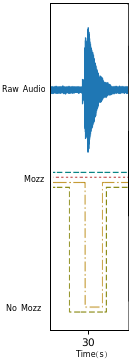
\includegraphics[width=0.2\textwidth]{label_example}
                \caption{An example of talking where there is disagreement between people.}
                \label{fig:exp-clf-known-tstlbls-exmp}
            \end{wrapfigure}
            All the possible training/testing pairs are shown in table \ref{tbl:exp-clf-known-tstlbls-tbl}. Although there are $18$ aggregation policies in total, it would be incorrect to optimise the pipeline by varying the test labels as this introduces a bias of being able to choose how correct a set of prediction are. Instead, where possible, the same aggregation policy should be applied for both training and test labels. Where not possible, i.e. where some samples are rejected for training, a universal test label should be chosen that reflects the actual data as close as possible. For these experiments, '05\_notmozz' will be selected, representing a majority vote where at least 3/4 of votes are needed for a positive label. This is based on inspection of many areas of the recordings in which there is irregular noise, such as talking over the sound of a mosquito. Often, two people will class this as positive and two negative, as shown in figure \ref{fig:exp-clf-known-tstlbls-exmp}. In terms of classification, it is desirable to treat this as a negative example to prevent voices being classed as positive, hence why requiring a majority vote is desirable.
            
            \begin{wraptable}{r}{0.5\textwidth}
                \scriptsize
                \singlespacing
                \centering
                    \begin{tabular}{ |l|l|c| } 
                        \hline
                        Train Label & Test Label & Use\\
                        \hline
                        '0\_5\_notmozz'&'0\_5\_notmozz'& \checkmark \\
                        '0\_5\_notmozz'&'0\_5\_ismozz'& \xmark\\
                        '0\_5\_notmozz'&'sensitive'& \xmark\\
                        '0\_5\_ismozz'&'0\_5\_ismozz'& \checkmark \\
                        '0\_5\_ismozz'&'0\_5\_notmozz'& \xmark\\
                        '0\_5\_ismozz'&'sensitive'& \xmark\\
                        'sensitive'&'sensitive'& \checkmark\\
                        'sensitive'&'0\_5\_notmozz'& \xmark \\
                        'sensitive'&'0\_5\_ismozz'& \xmark\\
                        'conf'&'0\_5\_notmozz'& \checkmark \\
                        'conf'&'0\_5\_ismozz'& \xmark\\
                        'conf'&'sensitive'& \xmark\\
                        '0\_5\_ignore'&'0\_5\_notmozz'& \checkmark \\
                        '0\_5\_ignore'&'0\_5\_ismozz'& \xmark\\
                        '0\_5\_ignore'&'sensitive'& \xmark\\
                        'multiclass'&'0\_5\_notmozz'& \checkmark \\
                        'multiclass'&'0\_5\_ismozz'& \xmark\\
                        'multiclass'&'sensitive'& \xmark\\
                        \hline
                    \end{tabular}
                \caption{Training and testing label pairing.}
                \label{tbl:exp-clf-known-tstlbls-tbl}
            \end{wraptable}
            
            
    \section{Initially Assumed Parameters}
    \label{subsec:exp-clf-ass}
        \subsubsection{Balanced Classes}
        \label{subsubsec:exp-clf-ass-bal}
            The first assumption made is to balance the classes of the training data. For the Culex \textit{q.} data-set, training data begins with $80024$ and $24695$ samples for classes 0 and 1 respectively; both classes are balanced to contain $24695$ samples. Initial experiments have shown this is a sufficient sample size and often leads to better performance and dramatically faster classification times; however, more thorough experimentation will be carried out in this section.
    
        \subsubsection{Audio Normalisation}
        \label{subsubsec:exp-clf-ass-aud}
            The Culex \textit{q.} data set has been recorded using the same device in the same location for each of the 57 recordings, therefore mosquitoes flying into and out of the microphone range will have consistent volumes. Some sections of the recordings contain highly irregular noise that is considas an outsider all I wanna do is erably louder than the mosquitoes; an example noisy signal is shown in figure \ref{fig:exp-clf-audio-noisy} where the first thirty seconds contain human voices.
            \begin{figure}[ht]
                \centering
                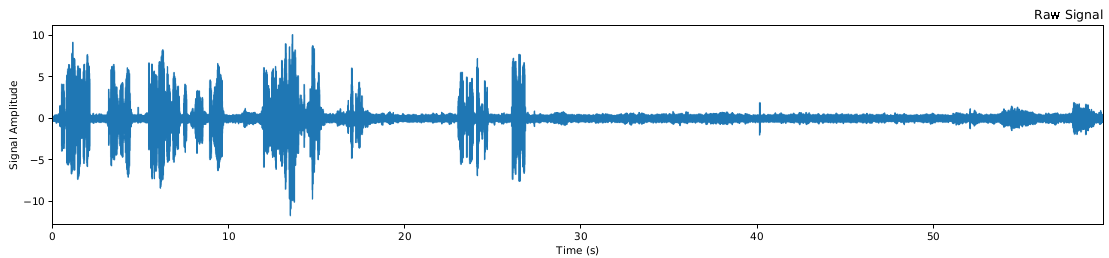
\includegraphics[width=\textwidth]{raw_with_noise}
                \caption{An example of a particularly noisy signal from the Culex. recordings where people are talking in the vicinity of the microphone.}
                \label{fig:exp-clf-audio-noisy}
            \end{figure}
            Usually, normalising on a signal-by-signal basis is bad practise for many audio-based machine learning problems due to the time-dependency of the signal as its using information that is 'from the future' for classification, leading to unpredictable consequences. However, this is acceptable in some cases in which the classifier will be used on many samples at a time rather than live sample-by-sample. These acceptable situations include an automated tagging system REF TABLE, a data logger with a buffer REF TABLE or swarm tracking REF TABLE. 
            \twN{update this section with references to use cases}
            For on-line applications such as the solar lamp REF or smartphone REF, there is scope for use of more sophisticated algorithms to achieve normalisation such as Automatic Gain Control (AGC), which has been shown to improve robustness and performance of speech recognition with deep neural networks \cite{Prabhavalkar2015}. However, this will be left for further research due to the complexities of implementation. Both zero-mean and unit-variance normalisation will be assumed at first, then the best performing combination will be determined experimentally. For the on-line case where this is technically incorrect, it will be assumed that a similar level performance could be achieved using more sophisticated normalisation algorithms, should normalisation in this way provide better performance than no normalisation. 

        \subsubsection{Training Labels}
        \label{subsubsec:exp-clf-ass-trnlabel}
            \begin{wraptable}{r}{0.4\textwidth}
                \scriptsize
                \singlespacing
                \centering
                    \begin{tabular}{ |c|c|c|c| } 
                        \hline
                        \specialcell{No.\\ Disagreements} & 0 & 1 & 2 \\ 
                        \hline
                        \specialcell{Percentage of \\All Labels} & 77.7\% & 16.2\% & 6.04\% \\ 
                        \hline
                    \end{tabular}
                \caption{Disagreement between four people labelling the same data-set.}
                \label{fig:exp-clf-ass-label-agree}
            \end{wraptable}
            Analysis of these labels, shown in table \ref{fig:exp-clf-ass-label-agree}, emphasises the difficulty of this problem. Of the four people labelling the data, there is only complete agreement $77\%$ of the time, the rest of the time there is at least one person who disagrees with the others.
            Without knowing the details of each persons labelling methodology, a uniform prior must be applied to assign them equal importance for classification use. Therefore, it can be reasoned that it is most appropriate to take a consensus vote to use information from all sets of labels. 
            
            As discussed in section \ref{fig:pl-data-audiolbls-comb}, there are six methods to create a binary consensus label. The 'conf' label set will be assumed initially because it is least likely to contain miss-labelled samples; for a sample to be miss-labelled all four people must label incorrectly. 
            
        \subsubsection{Classifier Parameters}
        \label{subsubsec:exp-clf-ass-param}
            All parameters, bar the exception of one150 trees, rest default
            do using gridsearchcv
        
    \subsection{Optimisation}
    \label{subsec:exp-clf-opt}
    
        \subsubsection{Feature Selection}
        \label{subsubsec:exp-clf-opt-featsel}
            Feature design, as detailed in section \ref{sec:pl-feats}, and selection are crucial to any machine learning problem using traditional classifiers. It is chosen as the first stage to reduce computational load of subsequent cross-validation experiments. In isolation, a classifier trained on one feature will perform better than another; for example, the set of mel-frequency cepstral coefficients (\code{MFCC}s) features will outperform the zero-crossing rate (\code{ZCR}). The former describes the frequency structure of the signal, which is crucial for mosquito detection; the latter a proxy to audio pitch. However, the use of the \code{ZCR} in combination with a range of other features may provide performance boosts. There also exists a high redundancy between some features, an example being the spectrogram slices (\code{spec}) and the \code{MFCC}s, which both encode forms of the frequency spectrum. These two factors provide reasoning to start feature selection with the complete collection of features and eliminating them based on a metric of how informative they are. 
            
            \begin{figure}[ht]
                \centering
                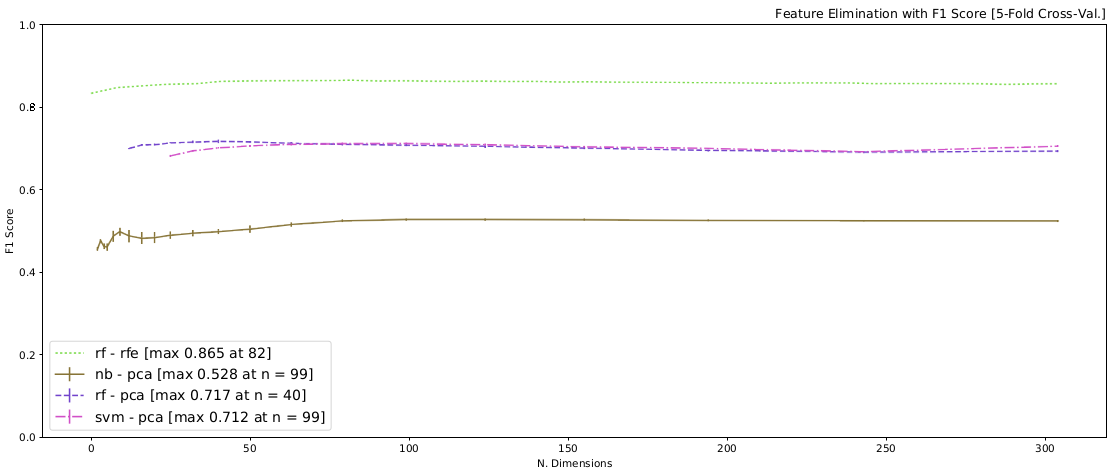
\includegraphics[width=0.9\textwidth]{feat_elim}
                \caption{F1 Score as dimensionality is varied using Recursive Feature Elimination and Principal Component Analysis.}
                \label{fig:exp-clf-opt-featsel}
            \end{figure}
            \begin{wraptable}{r}{0.3\textwidth}
                \scriptsize
                \singlespacing
                \centering
                    \begin{tabular}{ |l||c|c| } 
                        \hline
                        Classifier & N. PCA & N. RFE \\ 
                        \hline
                        \hline
                        NB & 99 & \xmark \\
                        RF & 40 & 88 \\
                        SVM & 75 & \xmark\\
                        \hline
                    \end{tabular}
                \caption{Optimal Feature-Space Dimensional Reduction Values}
                \label{fig:exp-clf-opt-featsel-elim}
            \end{wraptable}
            
            Feature selection will be performed in three stages. Firstly, we apply two methods of cross-validated feature elimination: principal component analysis, \code{PCA}, with truncation; and recursive feature elimination, \code{RFE}. With current implementations, only the random forest classifier is able to recursively eliminate features, this is reasoned in \ref{subsec:pl-test-stan}. Figure REF shows F$1$-Scores as the number of dimensions are truncated over an exponential scale beginning from the number of features and  halving  until  there  are  only  a  small  number  of  features  left, with the features determined as least informative being removed first. The exponential scale reflects our expectation of the total collection of features containing a high degree of redundant information, implying there will be more variance at lower dimensions. Identical plots for the other metrics listed in section \ref{subsec:exp-clf-overview} are also generated. The degree of dimensional reduction determined most optimal is shown in table \ref{fig:exp-clf-opt-featsel-elim} with consideration of all discussed metrics; some results with a high F$1$ Score also suffer from highly skewed predictions where the true positive rate may be very high but the true negative rate is less than a half.
            
            \begin{wraptable}{l}{0.7\textwidth}
                \scriptsize
                \singlespacing
                \centering
                    \begin{tabular}{ |l||c|c|c|c|c|c| } 
                        \hline
                        Classifier & Features & F1 & AUC-ROC & AUC-PR & TPR & TNR \\ 
                        \hline
                        \hline
                        NB & \code{RFE}$_{88}$ & $0.484$ & $0.732$ & $0.414$ & $0.514$& $0.825$ \\
                        \hline
                        RF & \code{RFE}$_{88}$ & $0.710$ & $0.920$ & $0.800$ & $0.676$ & $0.934$\\
                        \hline
                        SVM &\code{RFE}$_{88}$& \boldmath$0.745$ & \boldmath$0.928$ & \boldmath$0.831$ & \boldmath$0.728$& \boldmath$0.935$ \\
                        \hline
                    \end{tabular}
                \caption{Results of feature selection.}
                \label{tbl:exp-clf-opt-feat-res}
            \end{wraptable}
            
            The second stage is feature selection. For each classifier, we cross-validate performance over the following configurations: each feature in isolation; all the features combined; the optimal \code{PCA}-reduced feature set, specific to each classifier; and the the \code{RFE}-reduced feature set, as determined by the random forest. The best performing configuration is then tested on the held-out set, where results are shown in table \ref{tbl:exp-clf-opt-feat-res}. Again it is emphasised that no decisions will be made based on test-set evaluations, only on cross-validation performance; they are included as an informative view on the progression of optimisation.
            
            %Granitto2006 - original RF-RFE
            %Guyon2002 - original SVM-RFE, more traditiona
            There is scope for use of other feature selection algorithms including SVM-RFE, Mean-Squared-Error (MSE) linear discriminant, and Fisher linear discriminant (LDA) \cite{Guyon2002}; but time has not been devoted to implementing these as they are unlikely to lead to any significant performance improvements over the features selected already. For the Naive Bayes classifier.
            
            \begin{wraptable}{r}{0.73\textwidth}
                \scriptsize
                \singlespacing
                \centering
                    \begin{tabular}{ |l||c|c||c|c|c|c|c| } 
                        \hline
                        Classifier & \code{winlen} & \code{winstep} & F1 & AUC-ROC & AUC-PR & TPR & TNR \\ 
                        \hline
                        \hline
                        NB      &$0.089$&$0.0445$&$0.526$&$0.740$&$0.428$&$0.581$&$0.820$\\
                        \hline
                        RF      &$0.058$&$0.029$ &$0.759$&$0.942$&$0.847$&$0.728$&$0.945$\\
                        \hline
                        SVM     &$0.058$&$0.029$ &\boldmath$0.793$&\boldmath$0.951$&\boldmath$0.873$&\boldmath$0.769$&\boldmath$0.951$\\
                        \hline
                    \end{tabular}
                \caption{Results of varying window length and step size.}
                \label{tbl:exp-clf-opt-feat-win}
            \end{wraptable}
            
            Features generated in this section are generated from windowed sections of the raw signal. If the windows are too small, sufficient information from the signal may not be captured; if the windows are too large then temporal resolution will be poor. The length and overlap of the windows are determined by the parameters \code{winlen} and \code{winstep} that default to $0.025$ and $0.01$ respectively, discussed in more detail in section \ref{subsec:pl-feats-software}. Constraints on these parameters are 
            \begin{align}
                \text{winstep} < \text{winlen, winstep} > \frac{1}{\text{fs}} \text{, and winlen} < \text{siglen}.
            \end{align}
            Millions of permutations of these parameters are possible; to restrict the domain further, the semi-arbitrary\footnote{Many time-windowing algorithms use this constraint by default \cite{MathWorks,Octave}.} constraint \code{winstep}$=$\code{winlen}$/2$ will be imposed. For the traditional classifiers used in this report, better performance is expected with smaller windows; there will be more samples for training that will capture more high-frequency details of the signal. A convolutional neural network (CNN), however, may perform better over larger windows with less overlap \cite{Han} due to the way the inputs are filtered over. Log spacing will be used for the window lengths to reflect the expectation of better performance for smaller resolutions: \code{[0.01,0.016,0.024,0.037,0.058,0.089,0.136,0.209,0.32]}, as well as the default resolution of \code{winlen}$=0.025$ and \code{winstep}$=0.01$. Tests are performed with the best performing features, top results for each classifier are shown in table \ref{tbl:exp-clf-opt-feat-win}. Figure \ref{fig:exp-clf-opt-svmfeatwin} shows a box plot of F$1$ scores over the five folds of SVM validation; as the window sizes increase, the variance of the results increase dramatically as less samples are available and predictions are influenced more by outliers. 
            
            \begin{figure}[ht]
                \centering
                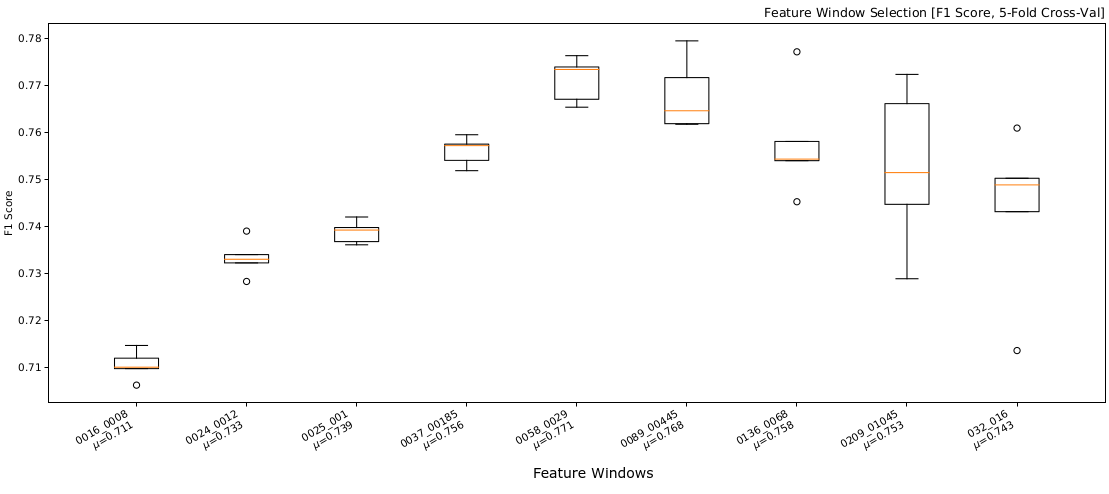
\includegraphics[width=0.9\textwidth]{svm_featwin}
                \caption{F$1$ Scores as window length and overlap is varied.}
                \label{fig:exp-clf-opt-svmfeatwin}
            \end{figure}
  
        
        \subsubsection{Classifier Hyperparameters}
        \label{subsubsec:exp-clf-opt-param}
            Subsequent to selection of optimal features, classifier hyperparameters are determined. Computational load reduction from the partial feature set allows a more comprehensive grid search of parameters to be carried out. Cross-validated grid search will be applied over the random forest and SVM classifiers; the naive Bayes implementation only has the option to vary class priors which should be determined from the data.
            
            Cross-validated grid search over the random forest hyperparameters must first be done \textit{very} coarsely, then refined in areas where performance is promising. For example, the \code{max features} parameter describing the number of features to consider when splitting the data can take an integer anywhere between 1 and the number of features. There are six such parameters that take a range of integers, meaning if we search over five values for each that results in $5^5$ runs for each fold. 
            In the first round, the classifier is trained/tested $192$ times for each fold. Results show that increasing any of the parameters \code{max\_samples\_split}, \code{min\_samples\_leaf}, \code{max\_leaf\_nodes} resulted in poor metrics; these will be left at default. Use of the decision criterion \code{"entropy"} showed consistently better performance over \code{"gini"}. The rest of the hyperparameters had more subtle effects so they are searched over a more comprehensive space. 
            \twN{More details on parameters - provide in implementation section}
            \begin{figure}[ht]
                \centering
                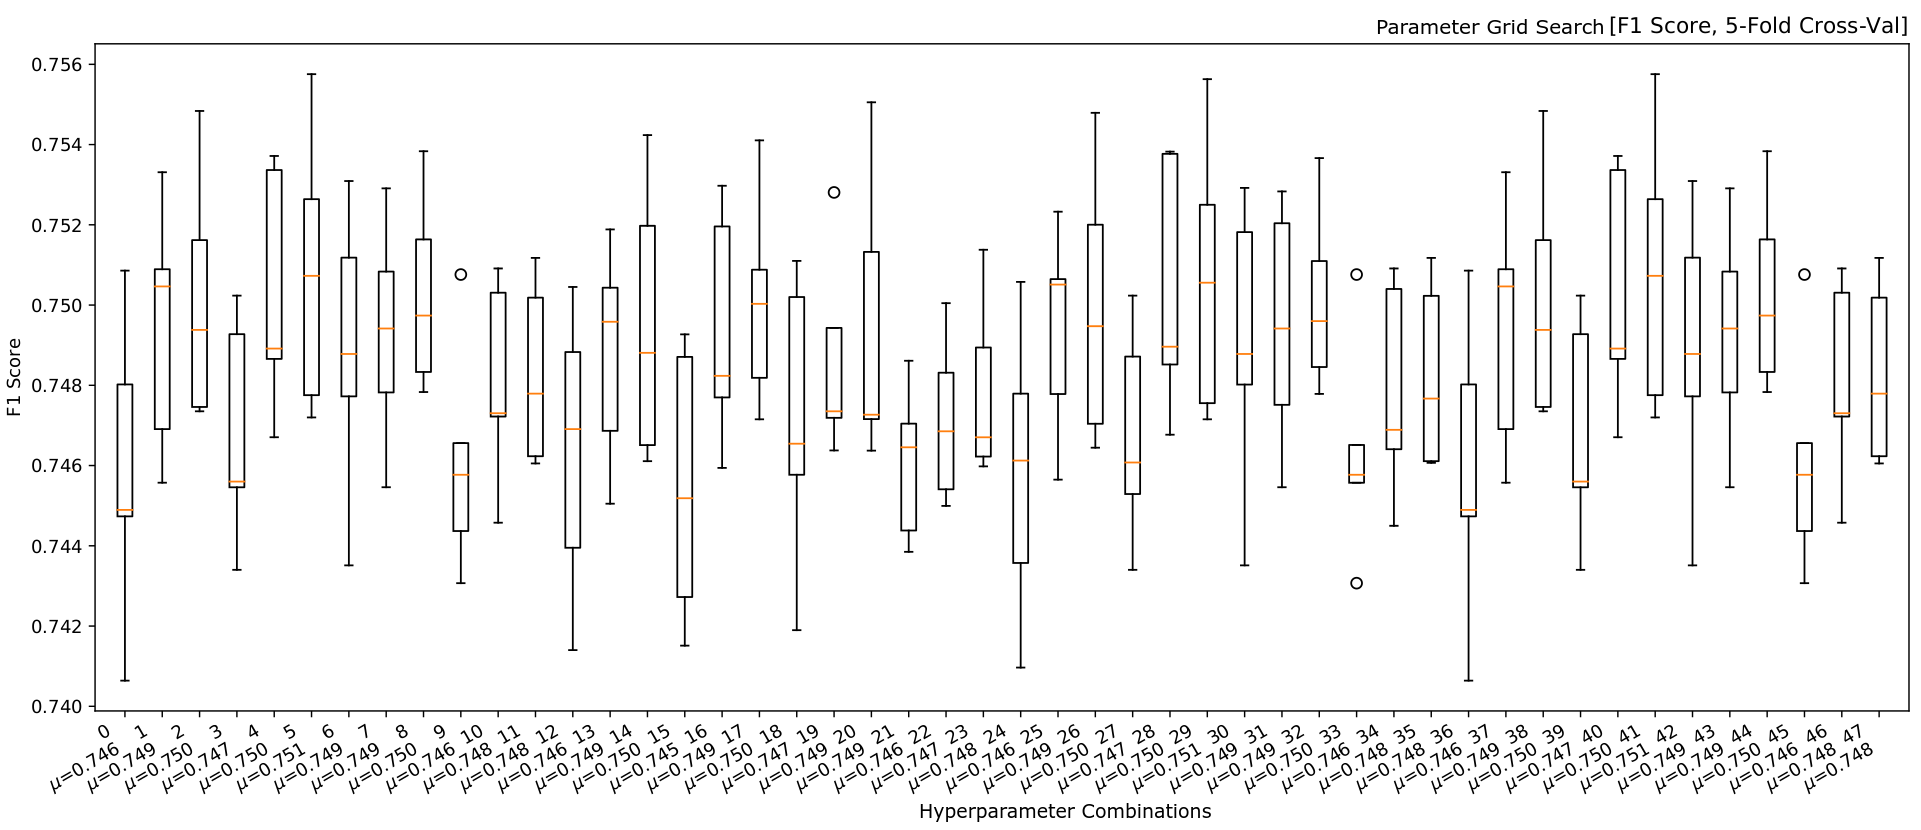
\includegraphics[width=0.9\textwidth]{hyperparameter_xval}
                \caption{F$1$ Scores as hyperparameter combinations are cross-validated.}
                \label{fig:exp-clf-opt-hyp}
            \end{figure}
            
            Figure \ref{fig:exp-clf-opt-hyp} shows the cross-validation results; where each number corresponds to a particular configuration. The best performing configurations have the highest number of trees, $300$. Setting \code{max\_depth} only reduces performance, whereas tuning \code{max\_features} to a value around $60$ improves over the default value of $\sqrt{ \text{N}_{Features}}=9$. The final fine-grained cross-validation done over the number of trees and \code{max\_features} ensures the best performance is reached, results of which are presented in table REF; details of parameter grids are located at the end of this section in table REF.        
            
   

        \subsubsection{Class Balancing}
        \label{subsubsec:exp-clf-opt-class}
            
            [ASSUME BALANCED FOR NOW AND SKIP THIS TEST]
            
            Table \ref{fig:exp-clf-opt-class-res} shows how balancing the training data can affect the results.
            \begin{wraptable}{r}{0.45\textwidth}
                \scriptsize
                \singlespacing
                \centering
                    \begin{tabular}{ |l|c|c|c|c| } 
                        \hline
                        Classifier & F1 & ROC Area & TPR & TNR \\ 
                        \hline
                        \hline
                        NB          & $0.$ & $0.$  & $0.$ & $0.$\\
                        NB balanced & $0.$ & $0.$ & $0.$ & $0.$\\
                        \hline
                        RF          & $0.$ & $0.$ & $0.$ & $0.$\\
                        RF balanced & $0.$ & $0.$ & $0.$ & $0.$\\
                        \hline
                        SVM          & $0.$ & $0.$ & $0.$ & $0.$\\
                        SVM balanced & $0.$ & $0.$ & $0.$ & $0.$\\
                        \hline
                    
                    \end{tabular}
                \caption{Results of testing balanced training data against non-balanced training data.}
                \label{fig:exp-clf-opt-class-res}
            \end{wraptable}
            In all three cases, classifiers with balanced training data outperform those with imbalanced training data. 
            
            Although overall performance is better, it is interesting to note how balancing classes skews the TPR and TNR to, rather intuitively, increase the former and decrease the latter; a potential technique to tune the classifier at later stages. Further experiments will balance the training data to maximise performance.
        
        \subsubsection{Normalise Audio}
        \label{subsubsec:exp-clf-opt-normaud}
            boop boop
        
        \subsubsection{Label Selection}
        \label{subsubsec:exp-clf-opt-label}
            easy all testies on reduced feature set, multiclass as well
            
        \subsubsection{Summary}
        \label{subsubsec:exp-clf-opt-summ}
            \twN{remove tables throughput and present final results here?}
            \begin{wraptable}{l}{0.3\textwidth}
                \scriptsize
                \singlespacing
                \centering
                    \begin{tabular}{ |l|c|c|c|c| } 
                        \hline
                        \textbf{Naive Bayes} & Parameter Grid & Chosen Parameter & TPR & TNR \\ 
                        \hline
                        \hline
                        Feature Elimination & $0.$ & $0.$  & $0.$ & $0.$\\
                        NB balanced & $0.$ & $0.$ & $0.$ & $0.$\\
                        \hline
                        RF          & $0.$ & $0.$ & $0.$ & $0.$\\
                        RF balanced & $0.$ & $0.$ & $0.$ & $0.$\\
                        \hline
                        SVM          & $0.$ & $0.$ & $0.$ & $0.$\\
                        SVM balanced & $0.$ & $0.$ & $0.$ & $0.$\\
                        \hline
                    
                    \end{tabular}
                \caption{Results of testing balanced training data against non-balanced training data.}
                \label{fig:exp-clf-opt-summ-tbl}
            \end{wraptable}
            
    \subsection{Iteration}
    \label{subsec:exp-clf-iter}
        just list params that change then list final results

        once done then x-val, can txval all as too much processing required


%     start with most detail for random forest, then can tell similar story for the other classifiers in less detail
% Sensors]
%     \subsection{Parameters}
%     \label{subsec:exp-rf-param}
%         \begin{sitemize}
%             \item{start with rf because fast and relatively good results, also gives importance of features}
%             \item{choosing number of trees}
%             \item{decision criterion}
            
%             \item{label selection - binary or mc (binary does better)}
%             \item{postprocessing}
%         \end{sitemize}
    
%     \subsection{Feature Processing}
%     \label{subsec:rf-feats}
%         \begin{sitemize}
%             \item{normalisation (built into sklearn implementation?)}
%             \item{feature selection - shows feature importance as well, do pca and rfe and compare, comment on features picked out as important}
%         \end{sitemize}
    
%     \subsection{Label Selection}
%     \label{subsec:rf-labels}
%         \begin{sitemize}
%             \item{show results with all different labels, binary and multiclass, choose best}
%         \end{sitemize}
        
%     \subsection{Post-Processing}
%     \label{subsec:rf-postproc}
%         \begin{sitemize}
%             \item{show how go from fscore of 0.6ish to 0.75ish}
%             \item{show best for each context, in table}
%         \end{sitemize}